%%%%%%%%%%%%%%%%%%%%%%%%%%%%%%%%%%%%%%%%%%%%%%%%%%%%%%%%%%%%%%%%%%%%%%%%%%%%%%%%%%
\begin{frame}[fragile]\frametitle{}
\begin{center}
{\Large Exponentials}
\end{center}
\end{frame}



%%%%%%%%%%%%%%%%%%%%%%%%%%%%%%%%%%%%%%%%%%%%%%%%%%%%%%%%%%%
 \begin{frame}[fragile]\frametitle{Power}
\begin{itemize}
\item $3 \times 3 = 3^2 = 9$
\item $3 \times 3 \times 3 = 3^3 = 27$
\item $4^7 = 16384$ here,  4 is the base, and 7 is the power or exponent in this expression.
\item The 'raised to' can be seen as whole number.
\item Can it be a fraction?
\item Can it be negative?
\end{itemize}
\end{frame}

%%%%%%%%%%%%%%%%%%%%%%%%%%%%%%%%%%%%%%%%%%%%%%%%%%%%%%%%%%%
 \begin{frame}[fragile]\frametitle{Radicals (Roots)}

\begin{itemize}
\item Sometimes you'll need to calculate one or other of the elements themselves.
\item $?^2 = 9$
\item This expression is asking, given a number (9) and an exponent (2), what's the base? 
\item In other words, which number multiplied by itself results in 9? 
\item This type of operation is referred to as calculating the root, and in this particular case it's the square root $\sqrt 9 = 3$ 
\item $36^{1/2} =?$
\item $81^{1/3} =?$
\end{itemize}
\end{frame}

%%%%%%%%%%%%%%%%%%%%%%%%%%%%%%%%%%%%%%%%%%%%%%%%%%%%%%%%%%%
 \begin{frame}[fragile]\frametitle{Radicals (Roots)}
\begin{lstlisting}
import math

# Calculate square root of 25
x = math.sqrt(25)
print (x)

# Calculate cube root of 64
cr = round(64 ** (1. / 3))
print(cr)
\end{lstlisting}
\end{frame}


%%%%%%%%%%%%%%%%%%%%%%%%%%%%%%%%%%%%%%%%%%%%%%%%%%%%%%%%%%%
 \begin{frame}[fragile]\frametitle{Logarithms}

\begin{itemize}
\item To determine the exponent for a given number and base. 
\item In other words, how many times do I need to multiply a base number by itself to get the given result.
\item $4^x =16$, what is $x$?
\item Such solutions are found by logarithms
\item $x = \log_4 (16) = 2$
\item Log finds the POWER to given base, of a number.
\item Whats Log of 1000 to base 10?
\end{itemize}
\end{frame}

%%%%%%%%%%%%%%%%%%%%%%%%%%%%%%%%%%%%%%%%%%%%%%%%%%%%%%%%%%%
 \begin{frame}[fragile]\frametitle{Logarithms}
\begin{lstlisting}
import math

# Natural log of 29
print (math.log(29))

# Common log of 100
print(math.log10(100))
\end{lstlisting}
\end{frame}


%%%%%%%%%%%%%%%%%%%%%%%%%%%%%%%%%%%%%%%%%%%%%%%%%%%%%%%%%%%
 \begin{frame}[fragile]\frametitle{Logarithms}
\begin{itemize}
\item We know of log to base 10 and those log tables. But is there  a function/formula?
\item What is a log? Is it defined for all real values?
\item $10^{2.3} = 10^{\frac{23}{10}}$ Thats 10th root of $10^{23}$
\item $10^{-0.07} = \frac{1}{10^{0.07}}$
\item $10^{\sqrt{2}} = 10^{(2^{1/2})}$. Need to approximate $\sqrt{2}$ to some decimal places and then evaluate.
\item $10^x= y$ then $\log y = x$
\item $x$ can be any real number and $y$ will be corresponding unique number.
\end{itemize}
\end{frame}


%%%%%%%%%%%%%%%%%%%%%%%%%%%%%%%%%%%%%%%%%%%%%%%%%%%%%%%%%%%
 \begin{frame}[fragile]\frametitle{Logarithm to base $e$}
\begin{itemize}
\item $\log x = \int_1^x \frac{1}{t} dt$
\item Its area under curve from 1 to $x$. At $x=1$ there is no area thus $\log 1 = 0$
\begin{center}
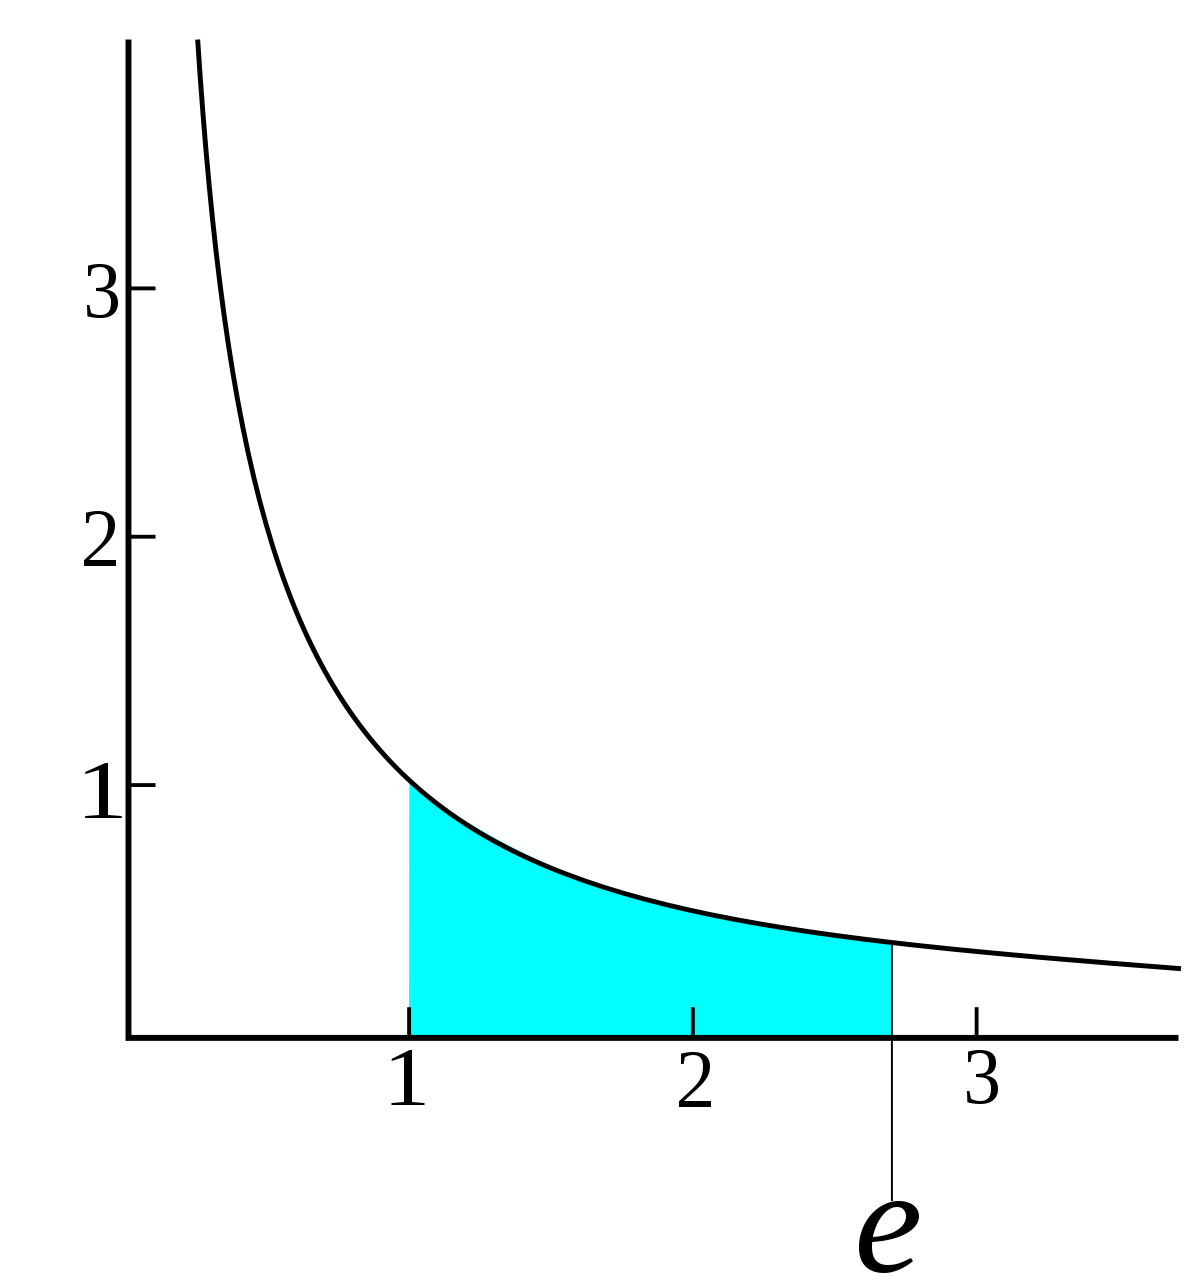
\includegraphics[width=0.4\linewidth,keepaspectratio]{ln}
\end{center}
\item At some $x$ where area is 1, is called as $e$.
\end{itemize}
\end{frame}


%%%%%%%%%%%%%%%%%%%%%%%%%%%%%%%%%%%%%%%%%%%%%%%%%%%%%%%%%%%
 \begin{frame}[fragile]\frametitle{Rules}
Add/Subtract with same power terms
\begin{itemize}
\item We can add coefficients of same power terms
\item $x^2 + 3x^2$ is possible = $4x^2$
\end{itemize}
\end{frame}

%%%%%%%%%%%%%%%%%%%%%%%%%%%%%%%%%%%%%%%%%%%%%%%%%%%%%%%%%%%
 \begin{frame}[fragile]\frametitle{Rules}
Multiply
\begin{itemize}
\item Adds the POWER terms
\item $2x^3 \times 4x^2 = ?$
\item $8x^5$
\item Similarly division is opposite
\item $6x^5 / 3x^2 = 2x^3$
\end{itemize}
\end{frame}

%%%%%%%%%%%%%%%%%%%%%%%%%%%%%%%%%%%%%%%%%%%%%%%%%%%%%%%%%%%
 \begin{frame}[fragile]\frametitle{Exercise}
Reduce $2y = 2x^4 (\frac{x^2 + 2x^2}{x^3})$
\end{frame}
%%%%%%%%%%%%%%%%%%%%%%%%%%%%%%%%%%%%%%%%%%%%%%%%%%%%%%%%%%%
 \begin{frame}[fragile]\frametitle{Solution}
$y = 3x^3$

\begin{lstlisting}
import pandas as pd

df = pd.DataFrame ({'x': range(-10, 11)})

df['y'] = 3*df['x']**3

from matplotlib import pyplot as plt

plt.plot(df.x, df.y, color="magenta")
plt.xlabel('x')
plt.ylabel('y')
plt.grid()
plt.axhline()
plt.axvline()
plt.show()
\end{lstlisting}
\end{frame}

%%%%%%%%%%%%%%%%%%%%%%%%%%%%%%%%%%%%%%%%%%%%%%%%%%%%%%%%%%%
 \begin{frame}[fragile]\frametitle{Plot}
 \begin{lstlisting}
     x     y
0  -10 -3000
1   -9 -2187
2   -8 -1536
3   -7 -1029
4   -6  -648
5   -5  -375
6   -4  -192
7   -3   -81
8   -2   -24
9   -1    -3
10   0     0
11   1     3
12   2    24
13   3    81
14   4   192
15   5   375
16   6   648
17   7  1029
18   8  1536
19   9  2187
20  10  3000
\end{lstlisting}

\end{frame}

%%%%%%%%%%%%%%%%%%%%%%%%%%%%%%%%%%%%%%%%%%%%%%%%%%%%%%%%%%%
 \begin{frame}[fragile]\frametitle{Plot}
\begin{center}
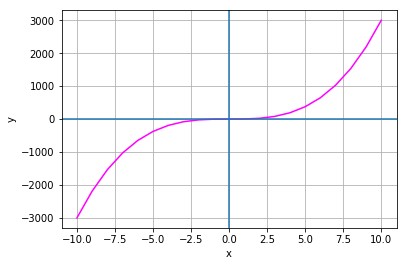
\includegraphics[width=0.8\linewidth,keepaspectratio]{log1}
\end{center}
\end{frame}


%%%%%%%%%%%%%%%%%%%%%%%%%%%%%%%%%%%%%%%%%%%%%%%%%%%%%%%%%%%
 \begin{frame}[fragile]\frametitle{Exercise}
$y = 2^x$

\begin{lstlisting}
import pandas as pd

df = pd.DataFrame ({'x': range(-10, 11)})

df['y'] = 2.0**df['x']

from matplotlib import pyplot as plt

plt.plot(df.x, df.y, color="magenta")
plt.xlabel('x')
plt.ylabel('y')
plt.grid()
plt.axhline()
plt.axvline()
plt.show()
\end{lstlisting}
\end{frame}

%%%%%%%%%%%%%%%%%%%%%%%%%%%%%%%%%%%%%%%%%%%%%%%%%%%%%%%%%%%
 \begin{frame}[fragile]\frametitle{Plot}
 \begin{lstlisting}
     x            y
0  -10     0.000977
1   -9     0.001953
2   -8     0.003906
3   -7     0.007812
4   -6     0.015625
5   -5     0.031250
6   -4     0.062500
7   -3     0.125000
8   -2     0.250000
9   -1     0.500000
10   0     1.000000
11   1     2.000000
12   2     4.000000
13   3     8.000000
14   4    16.000000
15   5    32.000000
16   6    64.000000
17   7   128.000000
18   8   256.000000
19   9   512.000000
20  10  1024.000000
\end{lstlisting}

\end{frame}

%%%%%%%%%%%%%%%%%%%%%%%%%%%%%%%%%%%%%%%%%%%%%%%%%%%%%%%%%%%
 \begin{frame}[fragile]\frametitle{Plot}
\begin{center}
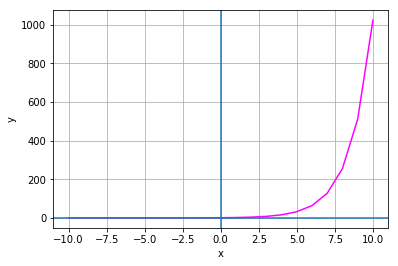
\includegraphics[width=0.8\linewidth,keepaspectratio]{log2}
\end{center}
\end{frame}


%%%%%%%%%%%%%%%%%%%%%%%%%%%%%%%%%%%%%%%%%%%%%%%%%%%%%%%%%%%
 \begin{frame}[fragile]\frametitle{Exercise}
Suppose you deposit Rs 100 in a bank account that earns 5\% interest per year. What would the balance of the account be in twenty years, assuming you don't deposit or withdraw any additional funds?

\begin{lstlisting}
import pandas as pd

# Create a dataframe with 20 years
df = pd.DataFrame ({'Year': range(1, 21)})

# Calculate the balance for each year based on the exponential growth from interest
df['Balance'] = 100 * (1.05**df['Year'])

#Display the dataframe
print(df)

# Plot the line
%matplotlib inline
from matplotlib import pyplot as plt

plt.plot(df.Year, df.Balance, color="green")
plt.xlabel('Year')
plt.ylabel('Balance')
plt.show()
\end{lstlisting}
\end{frame}

%%%%%%%%%%%%%%%%%%%%%%%%%%%%%%%%%%%%%%%%%%%%%%%%%%%%%%%%%%%
 \begin{frame}[fragile]\frametitle{Solution}
\begin{lstlisting}
    Year     Balance
0      1  105.000000
1      2  110.250000
2      3  115.762500
3      4  121.550625
4      5  127.628156
5      6  134.009564
6      7  140.710042
7      8  147.745544
8      9  155.132822
9     10  162.889463
10    11  171.033936
11    12  179.585633
12    13  188.564914
13    14  197.993160
14    15  207.892818
15    16  218.287459
16    17  229.201832
17    18  240.661923
18    19  252.695020
19    20  265.32977
\end{lstlisting}
\end{frame}

%%%%%%%%%%%%%%%%%%%%%%%%%%%%%%%%%%%%%%%%%%%%%%%%%%%%%%%%%%%
 \begin{frame}[fragile]\frametitle{Plot}
\begin{center}
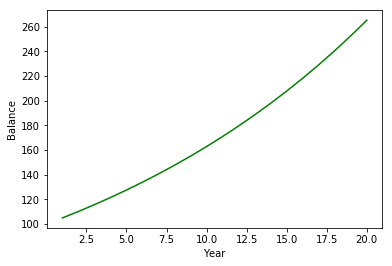
\includegraphics[width=0.8\linewidth,keepaspectratio]{log3}
\end{center}
\end{frame}
